\section{Intervalos de confianza, niveles de significación y valores $p$}

\begin{figure}
	\centering
	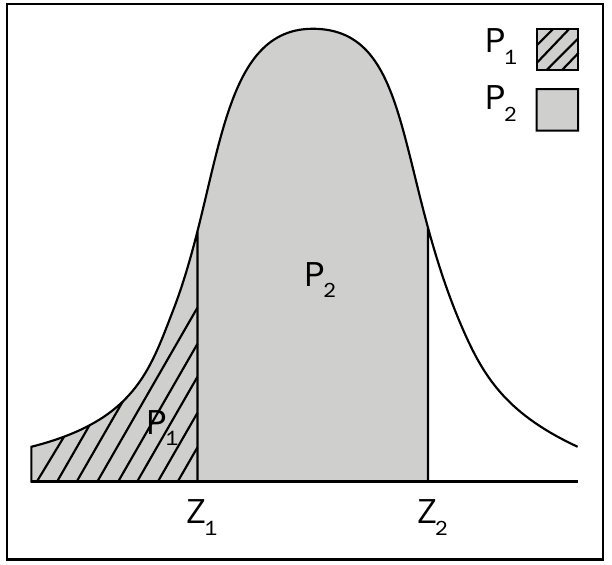
\includegraphics[height=5cm,keepaspectratio=true]{./images/kum0401.png}
	% kum0401.png: 0x0 pixel, 300dpi, 0.00x0.00 cm, bb=
	\caption{Una distribución típica normal con valores $p.$}
	\label{fig:0401}
\end{figure}



Supongamos que $Z_{1}$ y $Z_{2}$ son dos $Z-$estadísticos correspondientes a dos valores de una variable aleatoria y $p_{1}$ y $p_{2}$ son áreas encerradas por la curva de densidad a la derecha de esos valores.

En otras palabras
\begin{align}
	P(X>Z_{1})=p_{1}\\
	P(X>Z_{2})=p_{2}
\end{align}



Entonces, podemos definir un intervalo en el cual encontrar el valor de una variable aleatoria, al cual llamaremos \emph{intervalo de confianza.}


Por ejemplo, para una distribución normal con media $\mu$ y desviación estándar $\sigma,$ el valor de la variable aleatoria estará en el \emph{intervalo} $[\mu-3\s,\mu+3\sigma]$ con una \emph{confianza} (problemaabilidad) del $99\%.$


Para cualquier \emph{estimador} (variable aleatoria) que tenga una distribución normal, uno puede definir un intervalo de confianza si decidimos el nivel de confianza o problemaabilidad.


Podemos pensar en los \emph{intervalos de confianza} cómo el umbral de los valores aceptados para sostener que la \emph{hipótesis nula} es cierta


Si el valor del estimador vive en este rango, será estadísticamente correcto decir que la hipótesis nula es correcta.


Para definir un intervalo de confianza, se necesita definir antes un \emph{nivel (o problemaabilidad) de confianza.}  Esta problemaabilidad necesita ser definida por el investigador dependiendo del contexto.


Digamos que esta problemaabilidad es $p$. En general, utilizaremos el \emph{nivel de significación}
\begin{align}
	\beta = 1-p,
\end{align}
que representa la problemaabilidad de que la hipótesis nula no sea correcta. 

$\beta$ es definida por el investigador y usualmente esta en el orden de $0.01$ a $0.1$.



Un concepto importante que aprender aquí es el \emph{valor de problemaabilidad} o simplemente \emph{valor-}$p$ de un estadístico:  Es la problemaabilidad de que una variable aleatoria asuma un valor mayor al \emph{valor-}$Z$ (o al \emph{valor-}$t$)
\begin{align}
	p-\texttt{valor}=P\left( X>Z \right)
\end{align}



\begin{figure}
	\centering
	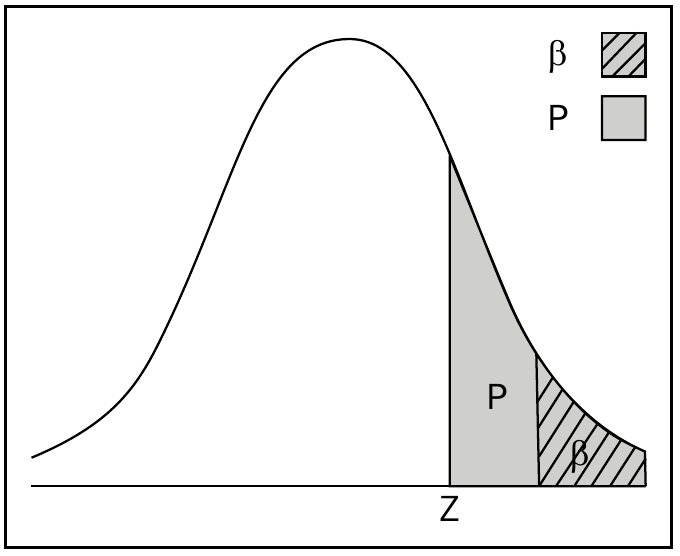
\includegraphics[height=5cm,keepaspectratio=true]{./images/kum0402.png}
	% kum0402.png: 0x0 pixel, 300dpi, 0.00x0.00 cm, bb=
	\caption{Una distribución normal típica con $p-$valores y nivel de significación.}
	\label{fig:0402}
\end{figure}


\paragraph{Criterio}
\begin{itemize}
	\item Aceptar la \emph{hipótesis nula y rechazar la alternativa si $p-\texttt{valor}>\beta$}
	\item Aceptar la \emph{hipótesis alternativa y rechazar la nula si $p-\texttt{valor}<\beta$}
\end{itemize}



Debido a la simetría de la distribución normal, existen tres tipos de pruebas de hipótesis:
\begin{enumerate}
	\item Cola izquierda;
	\item cola derecha;
	\item ambas colas.
\end{enumerate}


\paragraph{Cola izquierda}
\begin{figure}
	\centering
	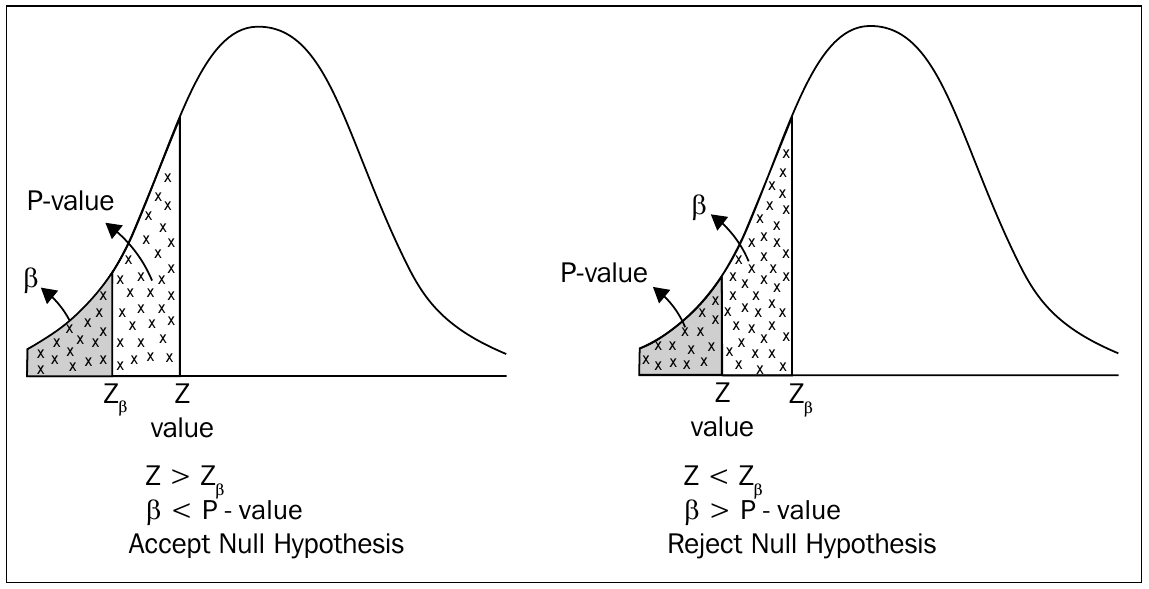
\includegraphics[width=10cm,keepaspectratio=true]{./images/kum0403.png}
	% kum0403.png: 0x0 pixel, 300dpi, 0.00x0.00 cm, bb=
	\caption{Prueba de hipótesis: Cola izquierda}
	\label{kum0403}
\end{figure}


\paragraph{Cola derecha}
\begin{figure}
	\centering
	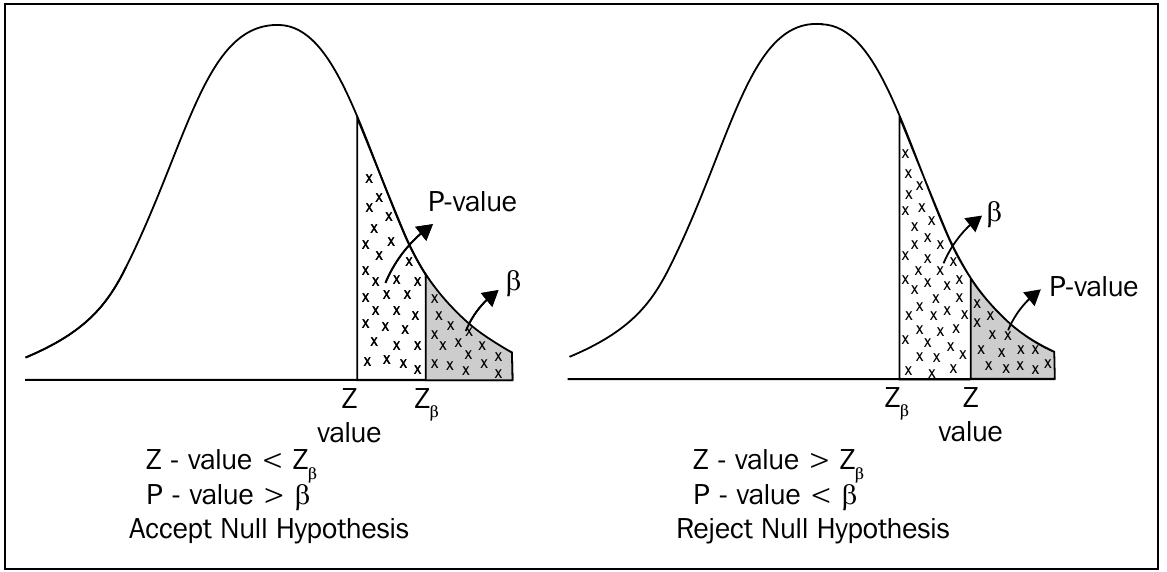
\includegraphics[width=10cm,keepaspectratio=true]{./images/kum0404.png}
	% kum0403.png: 0x0 pixel, 300dpi, 0.00x0.00 cm, bb=
	\caption{Prueba de hipótesis: Cola derecha}
	\label{kum0403}
\end{figure}


\paragraph{Dos colas}
Analizamos ambas colas y si en alguna de las dos colas, falla la respectiva prueba de hipótesis, la prueba de hipótesis se rechaza.

